\section{Обзор предметной области}
\label{sec:domain}

\subsection{Математическое понимание радиосигнала (1)}

Радиосвязь --- это разновидность беспроводной связи, где носителем сигнала является радиоволна. Передача и прием информации осуществляется посредством излучения и поглощения электромагнитных колебаний.
Передаваемые данные как правило неслучайны и могут быть представлена как функция от полезной информации и времени. В идеальных условиях было бы возможно, имея некоторые априорные знания о характере сигнала, безошибочно восстановить эту функцию и получить полезную информацию без потерь. Для примера можно рассмотреть стандартную запись сигнала с фазовой модуляцией (\autoref{eq:domain:pm_example}).

\begin{equation}
  \label{eq:domain:pm_example}
  s(t) = A_0 cos(\omega_0 t + m s_m(t))
\end{equation}
\begin{explanation}
\item[где] $s_m(t)$ --- полезная информация.
\end{explanation}

Но при распространении электромагнитной волны, она неизбежно испытывает влияние среды и изменяет свои параметры. Кроме того, вместе с целевым сигналом на приемник поступают множество шумовых. В результате полезную информацию можно восстановить только с определенной погрешностью.
Мгновенный уровень сигнала при этом непредсказуемо колеблется, поэтому в каждый момент времени его можно рассматривать как реализацию некоторой случайной величины, а развернутый во времени сигнал как случайный процесс. Такая абстракция очень полезна при статистическом анализе сигнала, так как позволяет использовать известные математические приемы при исследовании. Кроме того, его неизбежная составляющая --- фоновый шум --- обычно имеет нормальное распределение с нулевым математическим ожиданием.

Эта математическая модель обобщается на случай смесей сигналов и разладок (изменений параметров предполагаемого распределения). Также над случайными величинами определены математические операции: сложение, умножение и др. Это значит, что в терминах случайного процесса воспроизводимы как минимум элементарные преобразования сигналов.

\subsection{Типы сигналов (3)}

Полезная информация, передаваемая средствами радиосвязи имеет произвольные параметры и не годится для непосредственного использования как сигнал. Сначала она должна быть преобразована к желаемой полосе частот. Этот принцип позволяет использовать радио эфир с наибольшей эффективностью --- каждый передатчик работает на своей частоте и не мешает соседям.

Сигнал, заключенный в целевую полосу частот называется несущим, полезный сигнал --- модулирующим, а процесс кодирования модулирующего в несущий --- модуляцией. Для того применять методы их обнаружения необходимо понимать особенности встречаемых типов модуляции.


\subsubsection{Модулирующий сигнал.}\ В следующих пунктах будут рассмотрены характеристики различных способов модуляции. Чтобы ясно увидеть их отличия, зафиксируем модулирующий сигнал. Он был получен смесью трех синусоид с различными частотами и начальными фазами.

\begin{figure}[h]
  \centering
  \begin{subfigure}{0.45\textwidth}
    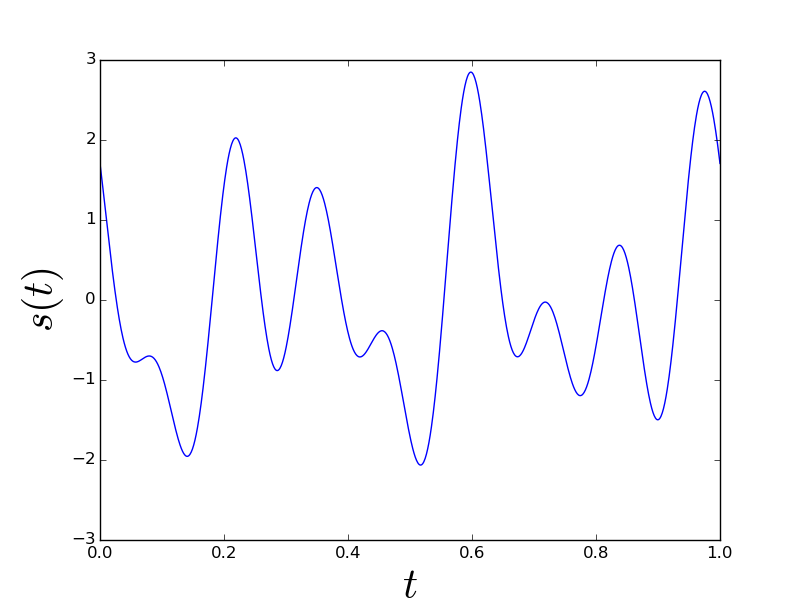
\includegraphics[width=\textwidth]{domain/modulator_example_time}
    \caption{}
  \end{subfigure}
  \begin{subfigure}{0.45\textwidth}
    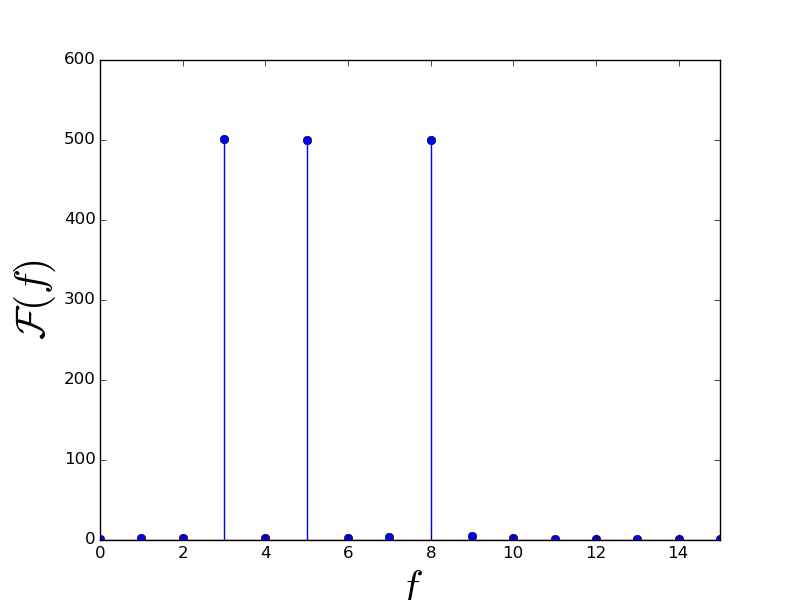
\includegraphics[width=\textwidth]{domain/modulator_example_freq}
    \caption{}
  \end{subfigure}
  \caption{Временная (а) и частотная (б) диаграммы модулирующего сигнала}
  \label{fig:domain:modulator}
\end{figure}

\subsubsection{Амплитудная модуляция (AM).}\ Амплитуда несущего сигнала изменяется в соответствии с модулирующим сигналом. AM активно применялась в первой половине \Romannum{20} века, в частности на гражданских радиостанциях. Однако, она очень неэффективна --- только треть мощности излучателя тратится на передачу информации, остальная часть нужна для передачи несущей. В результате в настоящее время заменена более совершенными методами и встречается редко. Ниже приведено выражение для амплитудной модуляции (\autoref{eq:domain:am}).

\begin{equation}
  \label{eq:domain:am}
  s(t) = A_0 (1 + m s_m(t)) cos(\omega_0 t + \phi_0)
\end{equation}
\begin{explanation}
\item[где] $A_0$ --- амплитуда несущей.
\item $m$ --- коэфициент модуляции.
\item $s_m(t)$ --- модулирующий сигнал.
\item $\omega_0$ --- частота несущей.
\item $\phi_0$ --- начальная фаза несущей.
\end{explanation}

\begin{figure}[h]
  \centering
  \begin{subfigure}{0.45\textwidth}
    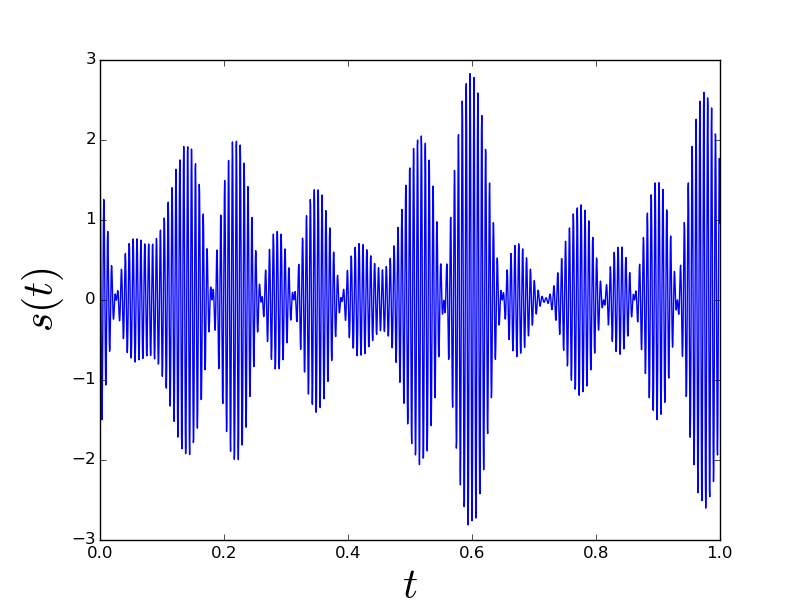
\includegraphics[width=\textwidth]{domain/am_example_time}
    \caption{}
  \end{subfigure}
  \begin{subfigure}{0.45\textwidth}
    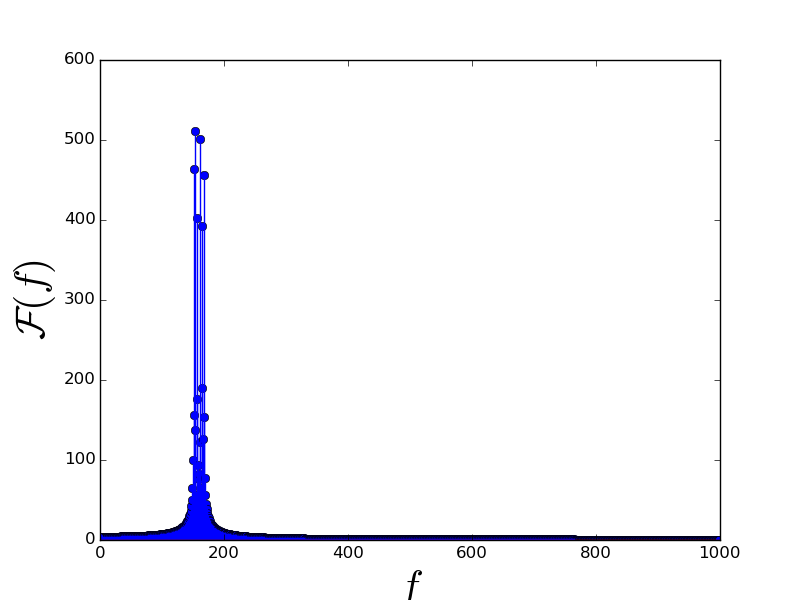
\includegraphics[width=\textwidth]{domain/am_example_freq}
    \caption{}
  \end{subfigure}
  \caption{Временная (а) и частотная (б) диаграммы амплитудно модулированного сигнала}
  \label{fig:domain:am}
\end{figure}

\subsubsection{Фазовая модуляция (PM).}\ Модулирующий сигнал воздействует на полную фазу несущей. Лишена недостатков AM, но на практике применяются только ее модификации. Временная диаграмма показывает, что мгновенная частота модулированного сигнала прямо пропорциональна производной по времени исходного. Так удобно, например, кодировать дискретные сигналы с высокой устойчивостью к аддитивным помехам. Однако, модулированный сигнал передает только изменение исходного, но не его самого. Если кодируется двоичная информация, то пропуск одного перехода повлечет инверсию все последующих бит. Формула PM приведена ниже (\autoref{eq:domain:pm}).

\begin{equation}
  \label{eq:domain:pm}
  s(t) = A_0 cos(\omega_0 t + m s(t))
\end{equation}
\begin{explanation}
\item[где] $A_0$ --- амплитуда несущей.
\item $\omega_0$ --- частота несущей.
\item $m$ --- девиация фазы.
\item $s_m(t)$ --- модулирующий сигнал.
\end{explanation}

\begin{figure}[h]
  \centering
  \begin{subfigure}{0.45\textwidth}
    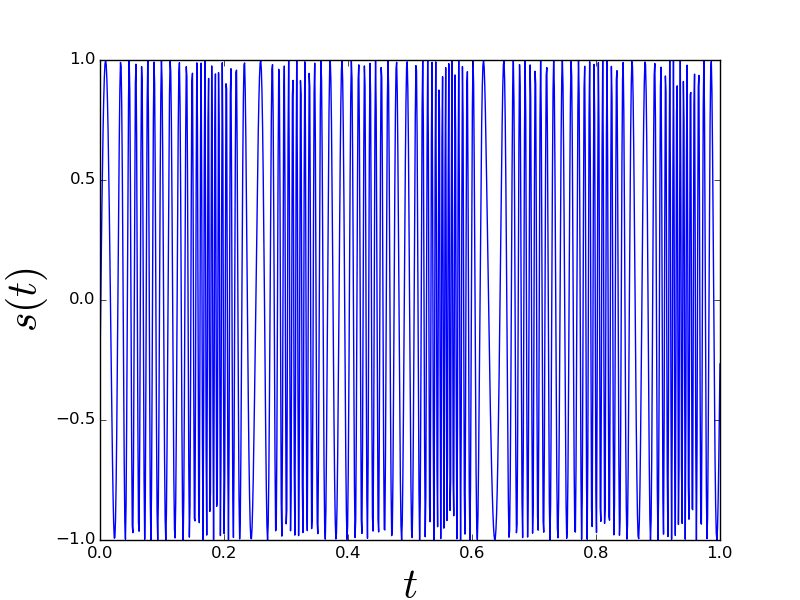
\includegraphics[width=\textwidth]{domain/pm_example_time}
    \caption{}
  \end{subfigure}
  \begin{subfigure}{0.45\textwidth}
    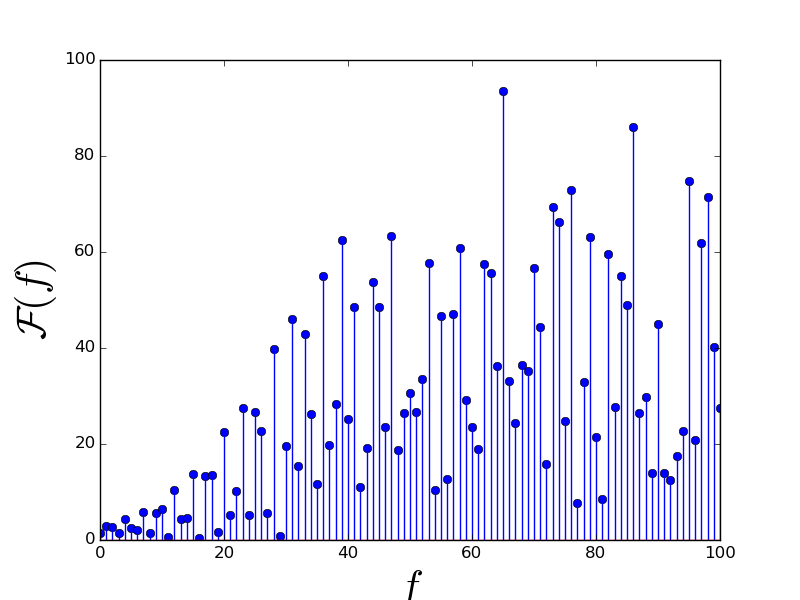
\includegraphics[width=\textwidth]{domain/pm_example_freq}
    \caption{}
  \end{subfigure}
  \caption{Временная (а) и частотная (б) диаграммы фазово модулированного сигнала}
  \label{fig:domain:pm}
\end{figure}


\subsubsection{Частотная модуляция (FM).}\ Модулирующий сигнал воздействует на мгновенную частоту несущей. Самый распространенный и известный тип модуляции. FM приобрела популярность из-за высокой помехоустойчивости (как и PM), высокого КПД передачи и эффективности использования выделенной полосы частот. Узкополосный режим позволяет разместить большое число передатчиков в ограниченном диапазоне частот (используется для служебной связи), а широкополосный --- значительно увеличить отношение мощности сигнала к шуму (используется в коммерческом радиовещании). Ниже приведено выражение для частотной модуляции (\autoref{eq:domain:fm}).

\begin{equation}
  \label{eq:domain:fm}
  s(t) = A_0 cos(\omega_0 t + \omega_d \int{s_m(t)dt}  + \phi_0)
\end{equation}
\begin{explanation}
\item[где] $A_0$ --- амплитуда несущей.
\item $\omega_0$ --- частота несущей.
\item $\omega_d$ --- девиация частоты.
\item $s_m(t)$ --- модулирующий сигнал.
\item $\phi_0$ --- начальная фаза несущей.
\end{explanation}

\begin{figure}[h]
  \centering
  \begin{subfigure}{0.45\textwidth}
    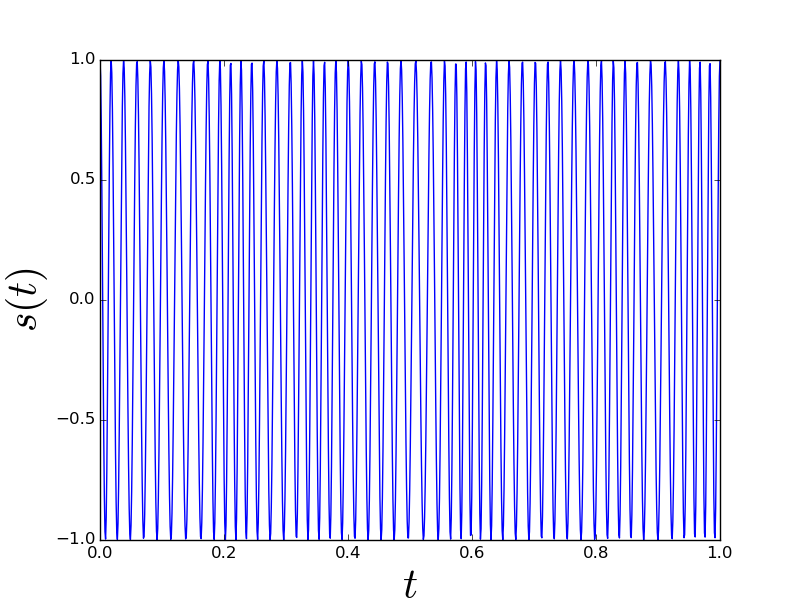
\includegraphics[width=\textwidth]{domain/fm_example_time}
    \caption{}
  \end{subfigure}
  \begin{subfigure}{0.45\textwidth}
    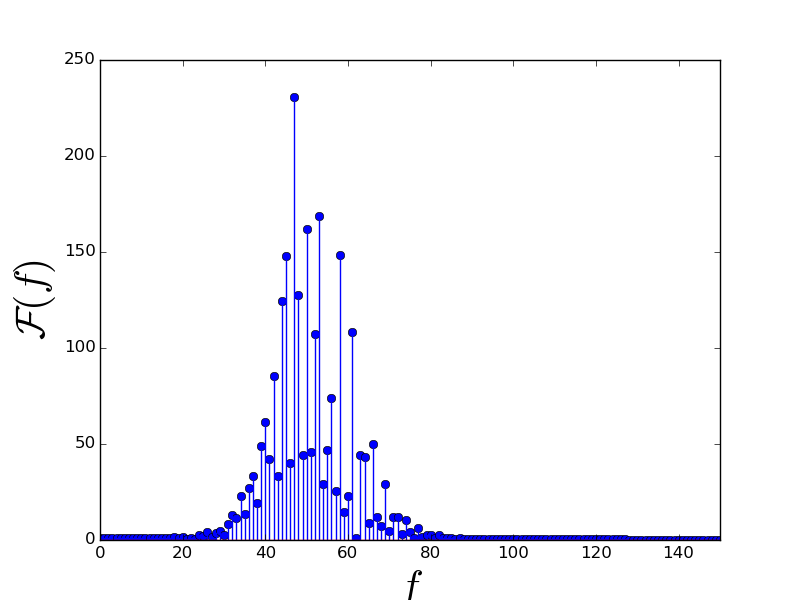
\includegraphics[width=\textwidth]{domain/fm_example_freq}
    \caption{}
  \end{subfigure}
  \caption{Временная (а) и частотная (б) диаграммы частотно модулированного сигнала}
  \label{fig:domain:fm}
\end{figure}

Рассмотренные выше методы являются фундаментальными --- они определяют три ключевых направления модуляции несущего сигнала. От них было порождено множество производных, устраняющих те или иные недостатки родителя.

Стоит упомянуть отдельно семейство методов, где модулирующим является дискретный сигнал. Цифровая модуляция даже получила отдельное название --- манипуляция. Она находит все большее применение в служебной и коммерческой связи из-за своей эффективности, помехоустойчивости и способности передавать цифровой сигнал без предварительного преобразования в аналоговую форму (это делается при модуляции). В данный момент на цифровую связь переведена большая часть служебных передач в городе Минске, а Норвегия объявила о намерении полностью заместить FM вещание на DAB и DAB+ \cite{norway_dab}.

Переход к новому способу связи это очень серьезное решение, так как старое оборудование не способно работать с новыми типами модуляции. Имеющиеся передатчики и приемники становятся совершенно бесполезными. Более того, страна, перешедшая на цифровой формат коммерческого вещания оказывается изолированной от передач соседей, если те работают в аналоге. Но какими бы страшными не казались проблемы миграции, технологический и как следствие экономический эффект в перспективе превышают расходы.

\subsection{Типы помех (2)}

В общем виде реальный сигнал можно рассматривать как совокупность передаваемого сигнала и воздействующих на него помех (\autoref{eq:domain:noise_types}).

\begin{equation}
  \label{eq:domain:noise_types}
  s(t) = k(t) e(t) + n(t)
\end{equation}
\begin{explanation}
\item[где] $e(t)$ --- передаваемый сигнал.
\item $k(t)$ --- коэффициент мультипликативной помехи.
\item $n(t)$ --- коэффициент аддитивной помехи.
\end{explanation}

Мультипликативные помехи возникают по причине изменения характеристик среды передачи с течением времени. Это может быть нагрев элементов радиосистемы, воздействие атмосферных явлений и др. Как правило, они действуют в течении длительного временного интервала и не мешают мгновенному приему и распознанию сигнала, поэтому опустим их подробное рассмотрение и сконцентрируемся на аддитивных помехах.

Аддитивные помехи представляют собой независимые добавки к принимаемому сигналу. Их разнообразие очень велико --- от реликтового излучения до преднамеренного зашумления эфира. Именно они могут оказывать существенное влияние на качество приема, поэтому стоит ознакомиться с их классификацией.

\subsubsection{По закону распределения}\ их разделяют на гауссовские и негауссовские. Такое деление удобно из-за того, что большая часть естественных помех подчиняется нормальному закону распределения. Это объясняется центральной предельной теоремой --- характер распределения суммы множества слабо взаимосвязанных помех, где ни одна не доминирует над остальными сходится к нормальному. Более того, часто можно принимать их математическое ожидание равным нулю. Негауссовские помехи учитывать сложнее, но обычно их тоже можно описывать случайным процессом с известным законом распределения.

\subsubsection{По характеру стационарности}\ выделяют стационарные и нестационарные помехи. Как и в теории случайных процессов, первые не изменяют характеристик своего распределения во времени, а вторые изменяют. В целях обнаружения сигнала часто предполагают, что помеха описывается стационарным случайным процессом с гауссовским законом распределения. Их также называют флуктуационные.

\subsubsection{По механизму возникновения}\ помехи разделяются на естественные, индустриальные, системные и искусственные.

Естественными помехами могут быть шумы в радиоприемном тракте, а также космические и атмосферные влияния. До нас непрерывно доходит шум Метагалактики, на фон которого накладываются излучения планет и звезд. Грозовая деятельность порождает еще один источник нежелательной активности в радиоэфире.

Индустриальные помехи создаются электрическими и электронными устройствами. Зачастую они носят импульсный характер: короткие всплески со сравнительно длительными периодами бездействия.

Системные помехи создаются другими радиотехническими средствами. Они также называются сосредоточенными, так как расположены в узком частотном интервале. Их могут вызвать близко расположенные радиостанции или большое число удаленных. Мешающее воздействие не обязательно объясняется перекрывающимися интервалами частот --- его причиной может быть отражение и рассеяние сигналов в атмосфере. Задача обеспечения электромагнитной совместимости сложна и пути ее решения описаны в отдельных научных работах.

Искусственные помехи создаются с целью мешающего действия радиосредствам. Использование таких форм помех в процессе военных действий является одной из форм "радиоэлектронной войны". Их формы очень разнообразны, но основная задача одна --- создание помехового фона, затрудняющего прием полезного сигнала или имитирование ложных целей.
\\

В целях дипломного проекта необходимо в первую очередь учитывать естественные флуктуационные помехи. Они всегда присутствуют в реальных условиях приема и могут быть описаны несложными математическими моделями. Иные типы помех встречаются достаточно редко и требуют специфических методов обработки.

\subsection{Комплексное представление сигнала (2)}
\subsection{Временной и частотный анализ (3)}
